
\section{Results}

Now we turn to discuss the results of our nuclear PDF fits.
%
First of all we show our main results, using EPS09 in the
determination of the conversion factors, and then
study the dependence on the input nuclear PDF set used
by comparing with using DSSZ as input.
%
We then to discuss the implications for the LHC heavy ion program,
by comparing our determination of the lead PDFs with other
recent nuclear PDF analysis available.



\subsection{NNPDFnucl1.0}

In Fig.~\ref{fig:nuclfact1}
we show the nuclear modifications factors of lead for the
  quark singlet $R_{\Sigma}(x,Q_0)$ (left plot) and for the
  gluon $R_{g}(x,Q_0)$ (right plot) at the input parametrization
  scale of $Q_0$=1 GeV for the NLO fit
  %
  The baseline proton PDF is NNPDF3.0 NLO and the
  EPS09 set
  has been used for the computation of the conversion factor.
  %
  The solid band indicates the one-sigma PDF uncertainty in the
  nuclear modification factors.

%%%%%%%%%%%%%%%%%%%%
\begin{figure}[t]
\begin{center}
 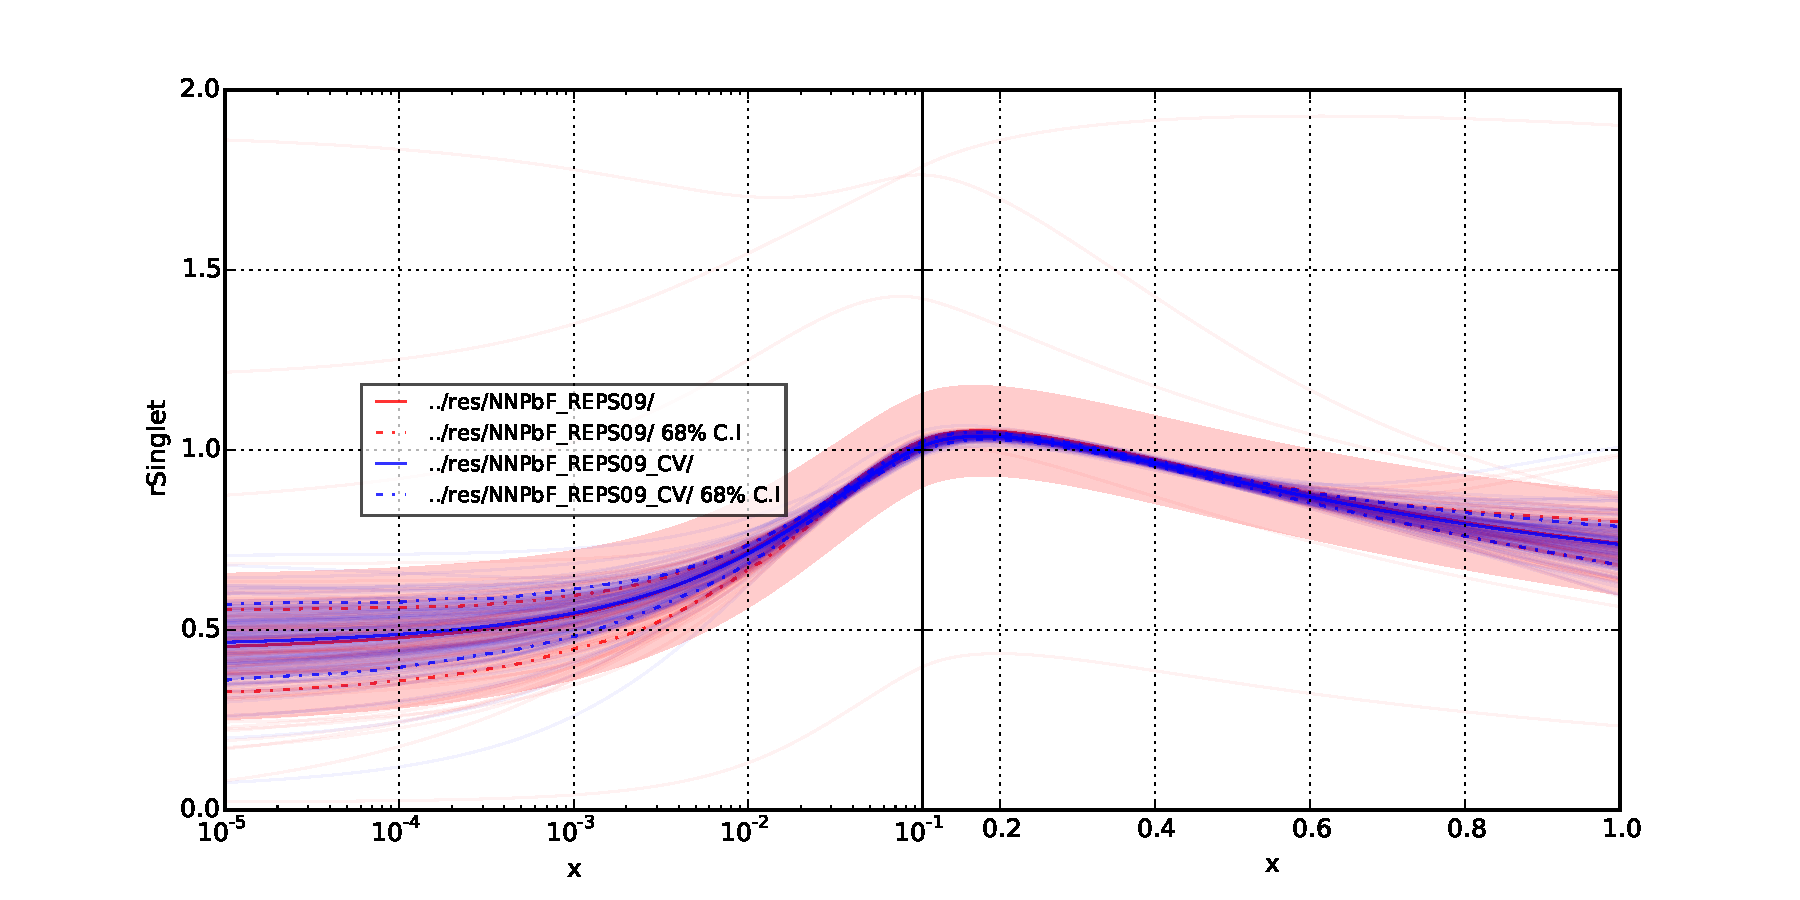
\includegraphics[width=0.49\textwidth]{plots/pdfcompSinglet-final1.pdf}
  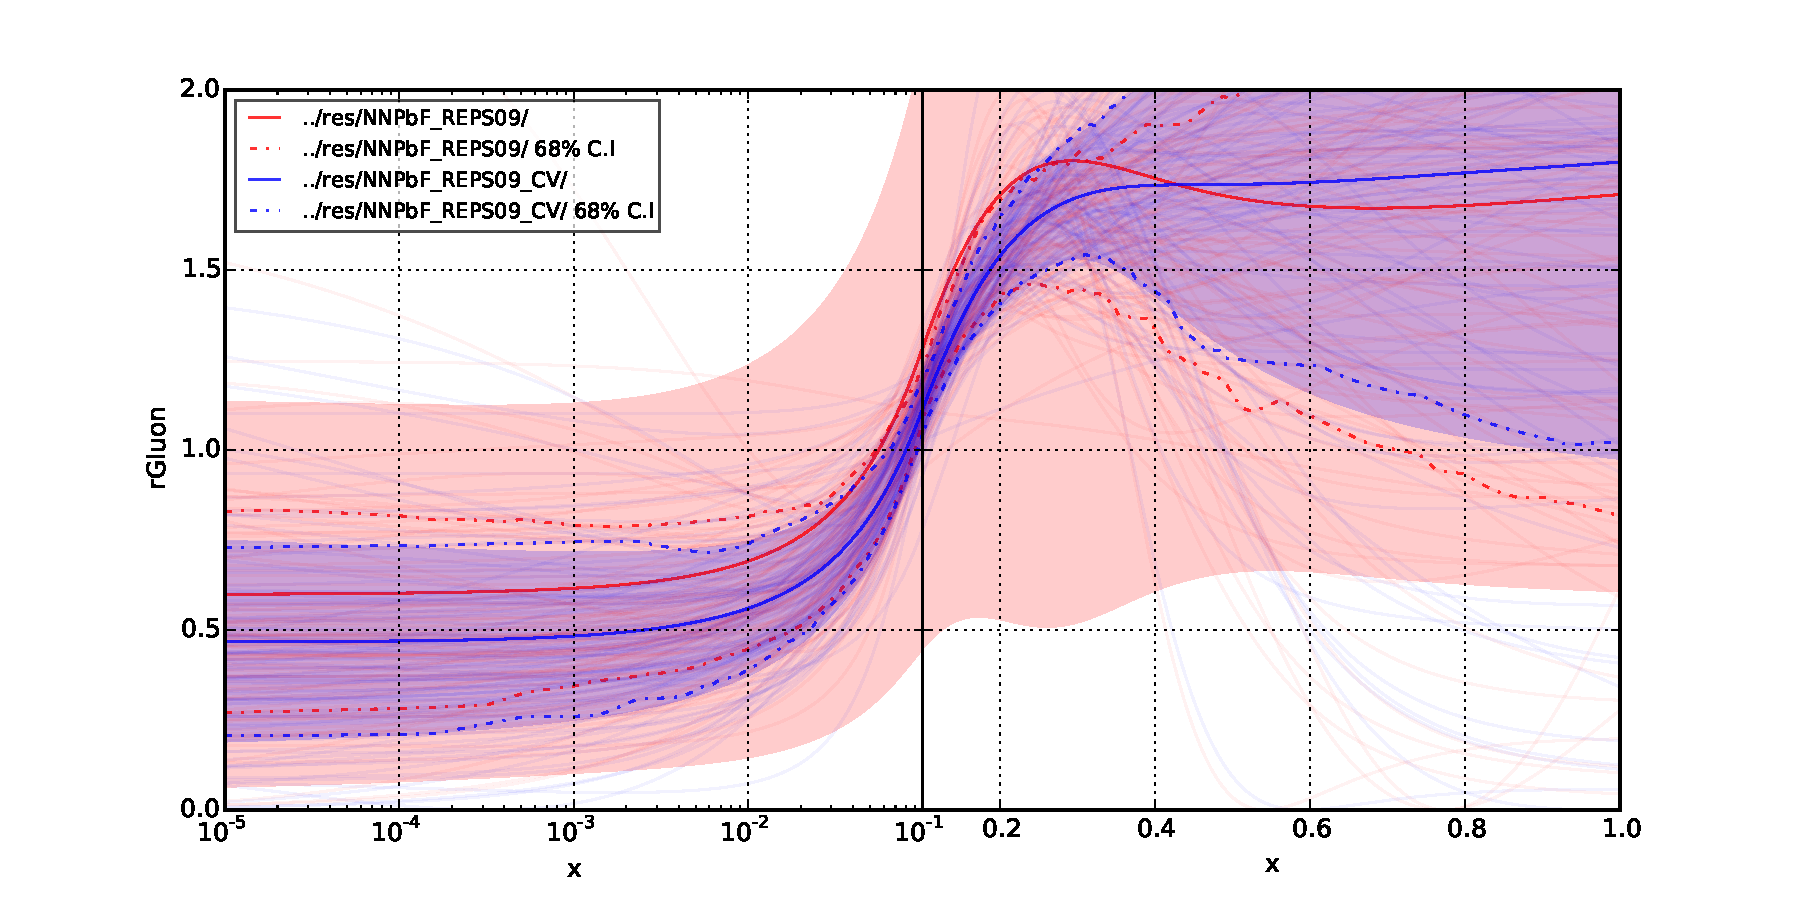
\includegraphics[width=0.49\textwidth]{plots/pdfcompGluon-final1.pdf}
 \end{center}
\vspace{-0.3cm}
\caption{\small The nuclear modifications factors of lead for the
  quark singlet $R_{\Sigma}(x,Q_0)$ (left plot) and for the
  gluon $R_{g}(x,Q_0)$ (right plot) at the input parametrization
  scale of $Q_0$=1 GeV for the NLO fit
  %
  The baseline proton PDF is NNPDF3.0 NLO and the
  EPS09 set
  has been used for the computation of the conversion factor.
  %
  The solid band indicates the one-sigma PDF uncertainty in the
  nuclear modification factors.
}
\label{fig:nuclfact1}
\end{figure}
%%%%%%%%%%%%%%%%%%%%%%%





\subsection{Dependence of the nuclear PDF set used for the conversion}

One critical aspect of our approach is the use of a nuclear
PDF set to perform the conversion of the nuclear DIS data
into a common observable $F_2^{\rm Pb}/F_2^{\rm d}$.
%
For our approach to be sound, the determination of the nuclear modification
factors $R_i^{\rm Pb}$ should be relatively independent
of the input PDF set used.
%
In this section we compare the results of fits using EPS09 in
the conversion with those of DSSZ, and show that a reasonable agreement
is found.
%
We also discuss how to combine into a single set the fits
obtained using the two nuclear PDF sets
as input.


In Fig.~\ref{fig:nuclfact2} we compare nuclear modification factors obtained using EPS09 as input
  with those obtained using DSSZ as input.
  %
  The solid bands correspond to the one-sigma
  PDF uncertainty, while the dot-dashed lines
  indicate the 68\% confidence level intervals.
  %
  As can be seen, the difference between the two determinations
  are always smaller than the PDF uncertainties.
  %
  As expected there are larger differences in the case of the
  gluon than for the singlet, though interestingly the qualitative
  behavior of the gluon modification factor is the same in the two
  cases.

  Note that in the case of DSSZ the number of fitted data points
  is smaller than in the case of EPS09, since the typically
  ;larger values of the PDF uncertainties sin the former
  lead to the cut Eq. to be applied more restrictively.
  %
  As expected, this leads to somewhat larger PDF uncertainties,
  specially at small-$x$.
  %
  We also note that the nuclear modification factors are relatively
  Gaussian in the data region, while as expected the distribution
  becomes non-Gaussian in the extrapolation region at small-$x$,
  where no experimental constraints are available.

  

%%%%%%%%%%%%%%%%%%%%
\begin{figure}[t]
\begin{center}
 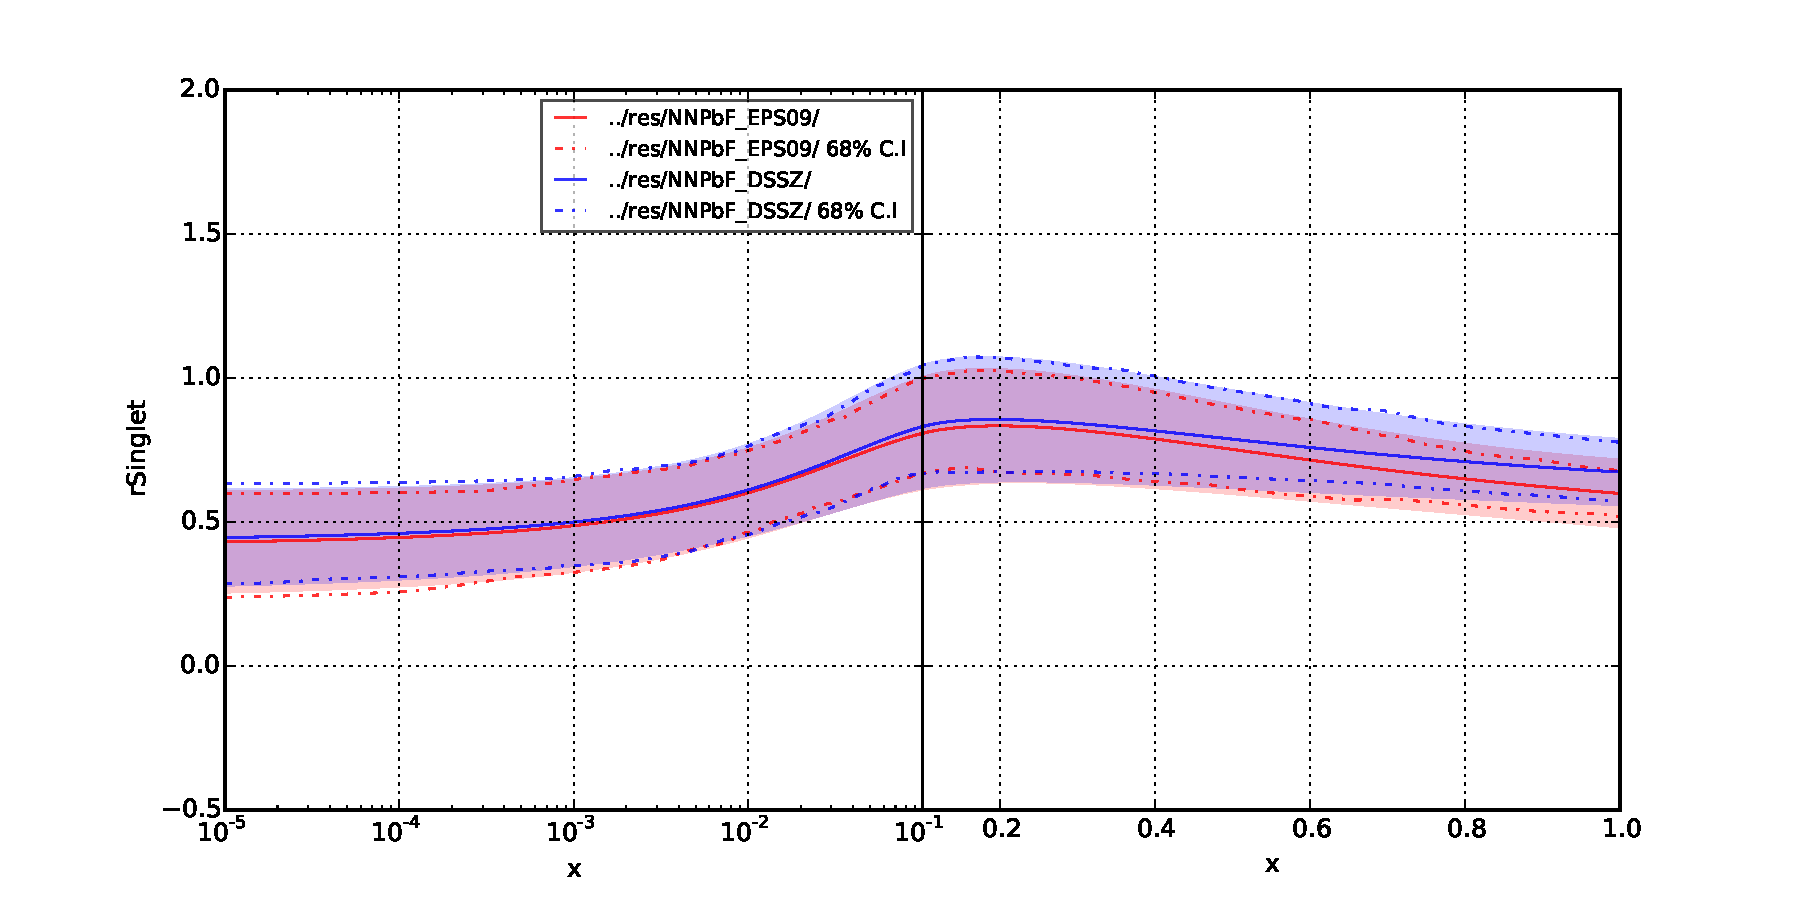
\includegraphics[width=0.49\textwidth]{plots/pdfcompSinglet-final2.pdf}
  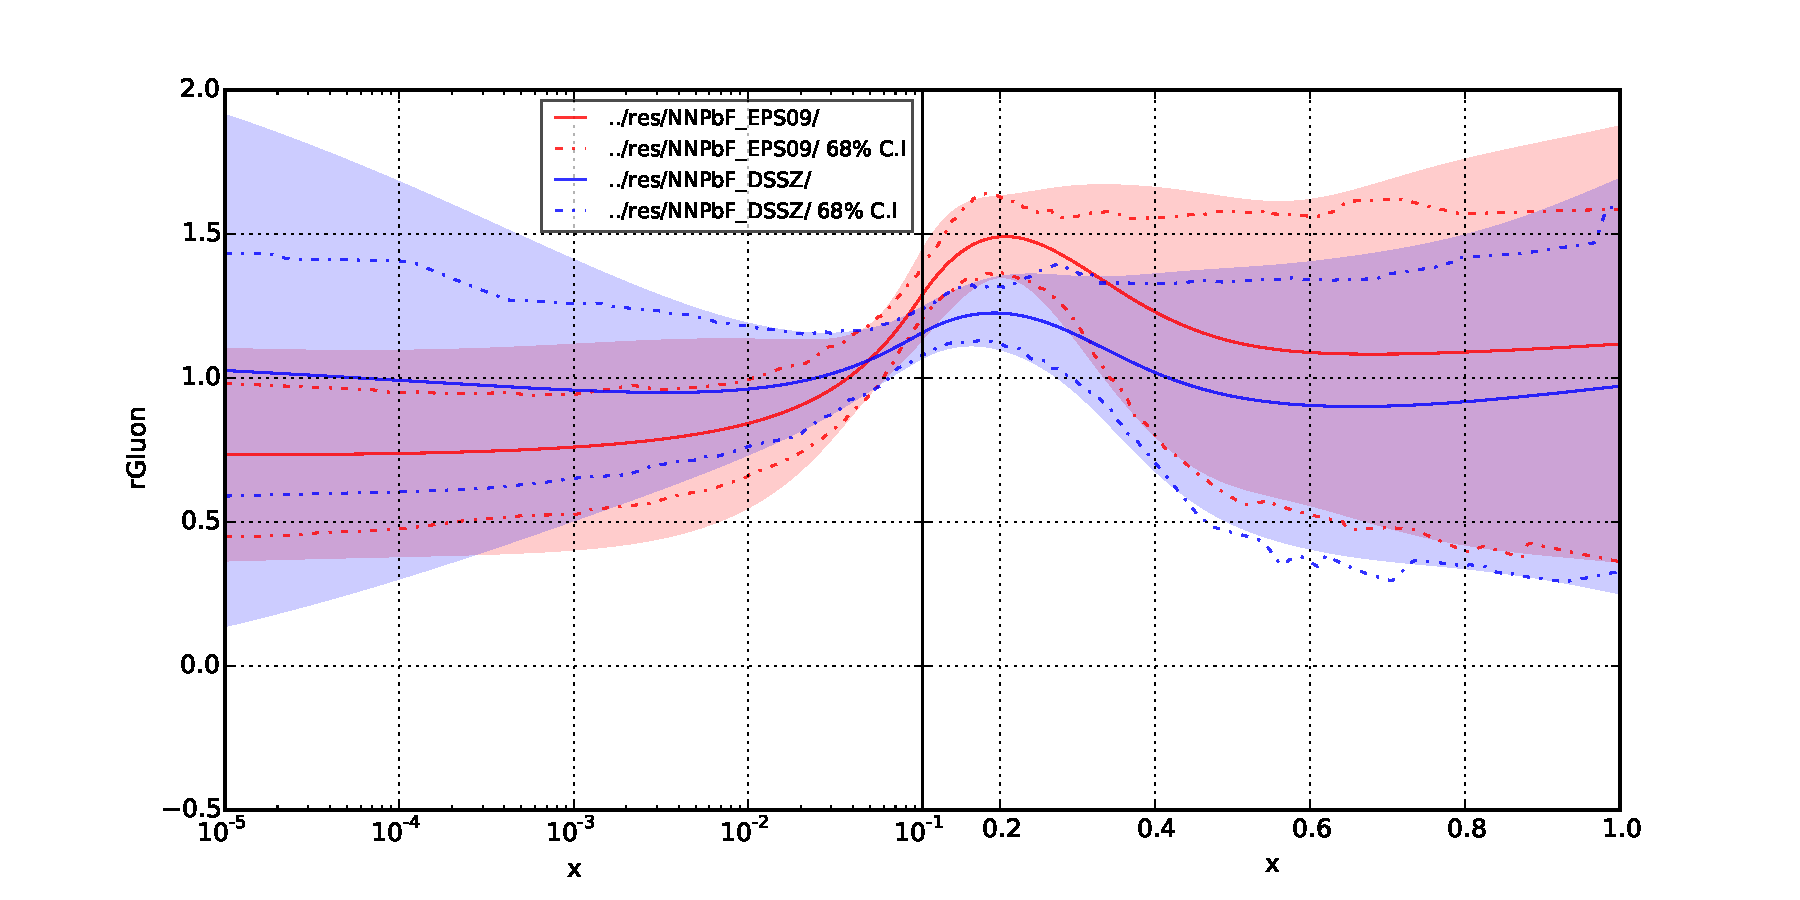
\includegraphics[width=0.49\textwidth]{plots/pdfcompGluon-final2.pdf}
 \end{center}
\vspace{-0.3cm}
\caption{\small Same as Fig.~\ref{fig:nuclfact1}, now comparing
  the nuclear modification factors obtained using EPS09 as input
  with those obtained using DSSZ as input.
  %
  The solid bands correspond to the one-sigma
  PDF uncertainty, while the dot-dashed lines
  indicate the 68\% confidence level intervals.
}
\label{fig:nuclfact2}
\end{figure}
%%%%%%%%%%%%%%%%%%%%%%%


MC-PDFs.
